% ============================================================
% Cours : Calcul matriciel
% Pôle Formation UIMM - CVDL - BTS ATI / CRSA - S. JAUBERT
% Référence programme : arrêté du 4 juin 2013, module « Calcul matriciel »
% (BTS ATI : p. 73-74 ; BTS CRSA : p. 97-98)
% ============================================================
\documentclass[a4paper,11pt]{article}
\usepackage[utf8]{inputenc}
\usepackage[T1]{fontenc}
% babel-french absent sur certains postes : chargement conditionnel
\IfFileExists{french.ldf}{\usepackage[french]{babel}}{\renewcommand{\contentsname}{Table des matières}}
\usepackage{helvet}
\usepackage{courier}
\renewcommand{\familydefault}{\sfdefault}
\usepackage[top=3cm, bottom=2.5cm, left=2cm, right=2cm, headheight=2cm]{geometry}
\usepackage{amsmath,amssymb,amsfonts}
\usepackage{graphicx}
\usepackage[dvipsnames,table]{xcolor}
\usepackage{tikz}
\usetikzlibrary{arrows.meta, calc, positioning, mindmap, matrix}
\usepackage[most]{tcolorbox}
\usepackage{fancyhdr}
\usepackage{hyperref}
\usepackage{enumitem}
\usepackage{booktabs,array,multicol,needspace}

\definecolor{uimmblue}{HTML}{005C85}
\definecolor{uimmred}{HTML}{D31326}
\definecolor{uimmlightblue}{HTML}{E8F1F8}
\definecolor{uimmgray}{HTML}{333333}
\definecolor{uimmlightgray}{HTML}{F5F5F5}
\hypersetup{colorlinks=true, linkcolor=uimmblue, urlcolor=uimmblue}

\usepackage{titlesec}
\titleformat{\section}
  {\LARGE\bfseries\color{uimmblue}}{\thesection.}{0.5em}{}[\vspace{2pt}{\color{uimmblue}\titlerule[1.5pt]}]
\titleformat{\subsection}{\Large\bfseries\color{uimmblue}}{\thesubsection.}{0.5em}{}
\titleformat{\subsubsection}{\large\bfseries\color{uimmblue!80!black}}{\thesubsubsection.}{0.5em}{}
\setlist[itemize,1]{label={\color{uimmblue}\textbullet}}
\setlist[itemize,2]{label={\color{uimmblue}--}}
\setlist[enumerate,1]{label={\color{uimmblue}\textbf{\arabic*.}}}

\newtcolorbox{definition}[1][]{colback=uimmlightblue, colframe=uimmblue,
  fonttitle=\bfseries\color{white}, title={\textsf{Définition}~#1}, coltitle=white,
  boxrule=1pt, arc=3pt, left=8pt, right=8pt, top=6pt, bottom=6pt, before skip=10pt, after skip=10pt}
\newtcolorbox{theoreme}[1][]{colback=uimmlightblue!50, colframe=uimmblue!80!black,
  fonttitle=\bfseries\color{white}, title={\textsf{Théorème / Propriété}~#1}, coltitle=white,
  boxrule=1.2pt, arc=3pt, left=8pt, right=8pt, top=6pt, bottom=6pt, before skip=10pt, after skip=10pt}
\newtcolorbox{methode}[1][]{colback=green!5, colframe=green!50!black,
  fonttitle=\bfseries\color{white}, title={\textsf{Méthode}~#1}, coltitle=white,
  boxrule=1pt, arc=3pt, left=8pt, right=8pt, top=6pt, bottom=6pt, before skip=10pt, after skip=10pt}
\newtcolorbox{exemple}[1][]{colback=orange!5, colframe=orange!70!black,
  fonttitle=\bfseries\color{white}, title={\textsf{Exemple}~#1}, coltitle=white,
  boxrule=1pt, arc=3pt, left=8pt, right=8pt, top=6pt, bottom=6pt, before skip=10pt, after skip=10pt,
  breakable}
\newtcolorbox{remarque}[1][]{colback=uimmlightgray, colframe=uimmgray,
  fonttitle=\bfseries, title={\textsf{Remarque}~#1}, boxrule=0.8pt, arc=3pt,
  left=8pt, right=8pt, top=6pt, bottom=6pt, before skip=10pt, after skip=10pt}
\newtcolorbox{appliindus}[1][]{colback=uimmred!5, colframe=uimmred!80!black,
  fonttitle=\bfseries\color{white}, title={\textsf{$\triangleright$ Application industrielle}~#1}, coltitle=white,
  boxrule=1.2pt, arc=4pt, left=8pt, right=8pt, top=6pt, bottom=6pt, before skip=10pt, after skip=10pt,
  breakable}
\newtcolorbox{attention}[1][]{colback=uimmred!5, colframe=uimmred,
  fonttitle=\bfseries\color{white}, title={\textsf{Attention}~#1}, coltitle=white,
  boxrule=1pt, arc=3pt, left=8pt, right=8pt, top=6pt, bottom=6pt, before skip=10pt, after skip=10pt}
\newtcolorbox{horsprog}[1][]{colback=white, colframe=uimmgray!60, borderline={0.6pt}{2pt}{uimmgray!60, dashed},
  fonttitle=\bfseries\color{uimmgray}, colbacktitle=uimmlightgray, title={\textsf{Pour aller plus loin (hors programme)}~#1},
  boxrule=0pt, arc=3pt, left=8pt, right=8pt, top=6pt, bottom=6pt, before skip=10pt, after skip=10pt}
\newtcolorbox{calculatrice}[1][]{colback=uimmlightblue!40, colframe=uimmblue,
  fonttitle=\bfseries\color{white}, title={\textsf{Fiche calculatrice}~#1}, coltitle=white,
  boxrule=1pt, arc=3pt, left=6pt, right=6pt, top=6pt, bottom=6pt, before skip=10pt, after skip=10pt}

% Raccourcis
\newcommand{\M}[1]{\begin{pmatrix}#1\end{pmatrix}}
\newcommand{\touche}[1]{\tikz[baseline=(k.base)]\node[draw=uimmgray, fill=white, rounded corners=1.5pt,
  inner sep=1.5pt, font=\footnotesize\sffamily](k){#1};}

\pagestyle{fancy}
\fancyhf{}
\renewcommand{\headrulewidth}{0pt}
\fancyhead[L]{\raisebox{-0.5\height}{
\includegraphics[height=1.5cm]{logo_uimm_placeholder.jpg}}}
\fancyhead[C]{\begin{minipage}{8cm}\centering
  {\small\color{uimmblue}\textbf{Pôle Formation UIMM - CVDL}}\\
  {\footnotesize\color{uimmgray} BTS ATI / CRSA -- Mathématiques}\end{minipage}}
\fancyhead[R]{{\small\color{uimmblue}\textbf{MOD12}}}
\fancyfoot[C]{{\color{uimmblue}\rule{\textwidth}{1pt}}\\[2pt]
  {\footnotesize\color{uimmgray} Pôle Formation UIMM -- Centre-Val de Loire \hfill S. JAUBERT \hfill \thepage}}

\begin{document}

\begin{titlepage}
\begin{tikzpicture}[remember picture, overlay]
  \fill[uimmblue] (current page.north west) rectangle ([yshift=-4cm]current page.north east);
  \node[anchor=north west] at ([xshift=2cm, yshift=-0.5cm]current page.north west)
    {
\includegraphics[height=3cm]{logo_uimm_placeholder.jpg}};
  \node[anchor=north east, white, font=\large\bfseries] at ([xshift=-2cm, yshift=-1.5cm]current page.north east)
    {Pôle Formation UIMM - CVDL};
  \node[anchor=north east, white, font=\small, align=right] at ([xshift=-2cm, yshift=-2.2cm]current page.north east)
    {BTS ATI / CRSA -- Mathématiques\\[2pt]S. Jaubert};
  \fill[uimmred] ([yshift=-4cm]current page.north west) rectangle ([yshift=-4.4cm]current page.north east);
  \node[anchor=center, text width=14cm, align=center] at ([yshift=-1cm]current page.center) {
    {\fontsize{28}{34}\selectfont\bfseries\color{uimmblue} Calcul matriciel}\\[20pt]
    {\Large\color{uimmgray} Module 12}\\[12pt]
    {\large\color{uimmgray}\textit{Matrices, opérations, puissances, inverse et systèmes linéaires}}\\[30pt]
    {\color{uimmblue}$\M{a_{11} & a_{12}\\ a_{21} & a_{22}}\times\M{x\\y}=\M{b_1\\b_2}
      \quad\Longleftrightarrow\quad X = A^{-1}B$}
  };
  \fill[uimmblue] ([yshift=1.5cm]current page.south west) rectangle (current page.south east);
  \node[anchor=center, white, font=\small] at ([yshift=0.75cm]current page.south) {
    Pôle Formation UIMM -- Centre-Val de Loire $\bullet$ La Fabrique de l'Avenir};
\end{tikzpicture}
\end{titlepage}

\thispagestyle{fancy}
\vspace*{0.1cm}
\begin{center}
{\LARGE\bfseries\color{uimmblue} MOD12 -- Calcul matriciel}\\[6pt]
{\large\color{uimmgray} Support de cours}\\[4pt]
{\normalsize\color{uimmgray} Auteur : S. JAUBERT \hspace{1cm} Formation : BTS ATI / CRSA}
\end{center}
\vspace{0.3cm}

\begin{tcolorbox}[colback=uimmlightblue!30, colframe=uimmblue,
  title={\textbf{\textsf{Fiche du Module}}}, fonttitle=\large\bfseries\color{white},
  coltitle=white, boxrule=1.2pt, arc=4pt, left=10pt, right=10pt, top=8pt, bottom=8pt]
\renewcommand{\arraystretch}{1.3}
\begin{tabular}{@{}>{\bfseries\color{uimmblue}}l @{\hspace{12pt}} p{12cm}@{}}
Bloc / Période : & Semestre 4 \\
Module :         & {[MOD12]} Calcul matriciel \\
Thème :          & Représenter une situation à plusieurs entrées et sorties par une matrice, calculer avec des matrices, modéliser un processus discret, résoudre un système linéaire par inversion \\
Référentiel :    & Arrêté du 4 juin 2013 (programme de mathématiques des BTS), module « Calcul matriciel ». Évalué en CCF, 2\textsuperscript{e} situation (BTS ATI, arrêté du 8 juillet 2024). \\
\end{tabular}
\end{tcolorbox}
\vspace{0.1cm}

\begin{tcolorbox}[colback=white, colframe=uimmblue!80!black,
  title={\textbf{\textsf{Séquences et Compétences travaillées}}}, fonttitle=\large\bfseries\color{white},
  coltitle=white, boxrule=1pt, arc=4pt, left=10pt, right=10pt, top=8pt, bottom=8pt]
\textbf{\color{uimmblue} [S01] -- Matrices et opérations}
\begin{itemize}[leftmargin=1.5cm]
  \item[\textbf{\color{uimmblue}[C01]}] Représenter une situation simple à l'aide d'une écriture matricielle
  \item[\textbf{\color{uimmblue}[C02]}] Effectuer des calculs matriciels (addition, multiplication par un réel, multiplication), à la main à l'ordre 2, à la calculatrice au-delà
  \item[\textbf{\color{uimmblue}[C03]}] Calculer une puissance de matrice et traiter un processus discret à l'aide d'une suite de matrices
\end{itemize}
\textbf{\color{uimmblue} [S02] -- Inverse d'une matrice et systèmes linéaires}
\begin{itemize}[leftmargin=1.5cm]
  \item[\textbf{\color{uimmblue}[C01]}] Montrer qu'une matrice est l'inverse d'une autre
  \item[\textbf{\color{uimmblue}[C02]}] Déterminer à l'aide d'une calculatrice ou d'un logiciel l'inverse d'une matrice inversible
  \item[\textbf{\color{uimmblue}[C03]}] Résoudre un système linéaire de $n$ équations à $n$ inconnues à l'aide d'une inversion de matrice
\end{itemize}
\end{tcolorbox}

\begin{remarque}[-- Positionnement du cours]
Prérequis : systèmes linéaires à deux inconnues (MOD00), suites (MOD02), probabilités (MOD08). Le programme impose les calculs \textbf{à la main sur des matrices d'ordre 2}. À l'ordre 3 ou plus, les calculs se font \textbf{à la calculatrice ou au logiciel}. La notion de déterminant n'est pas au programme.
\end{remarque}

\newpage
\tableofcontents
\newpage

% ============================================================
\needspace{7cm}
\section{Pourquoi des matrices ?}\label{sec:pourquoi}

\begin{tcolorbox}[colback=uimmlightblue!30, colframe=uimmblue, boxrule=0.8pt, arc=3pt,
  title={\textbf{\textsf{L'essentiel en une phrase}}}, fonttitle=\bfseries\color{white}, coltitle=white]
Une matrice est un \textbf{tableau de nombres} qui relie des \textbf{entrées} (ce qu'on consomme, ce qu'on commande, l'état de départ) à des \textbf{sorties} (ce qu'on produit, ce qu'on dépense, l'état d'arrivée). Le calcul matriciel fait en une seule opération ce qu'on ferait autrement ligne par ligne.
\end{tcolorbox}

\begin{appliindus}[-- Le fil rouge : l'atelier de vérins]\label{ex:filrouge}
Un atelier assemble trois modèles de vérins pneumatiques : $V_1$, $V_2$ et $V_3$. Chaque vérin consomme des tiges, des joints et des vis selon la \textbf{nomenclature} suivante.
\begin{center}
\renewcommand{\arraystretch}{1.3}
\begin{tabular}{|l|c|c|c|}
\hline
\rowcolor{uimmlightblue}
\textbf{Composant} \textbackslash\ \textbf{Vérin} & $V_1$ & $V_2$ & $V_3$ \\
\hline
Tige & 1 & 1 & 2 \\
\hline
Joint & 4 & 6 & 8 \\
\hline
Vis & 8 & 8 & 12 \\
\hline
\end{tabular}
\end{center}
La commande de la semaine est de $40$ vérins $V_1$, $25$ vérins $V_2$ et $10$ vérins $V_3$. Trois questions se posent au magasinier et au responsable de production :
\begin{enumerate}
  \item Combien de tiges, de joints et de vis faut-il sortir du stock ?
  \item Combien coûtent ces composants ?
  \item Le stock contient $85$ tiges, $390$ joints et $640$ vis. Combien de vérins de chaque modèle faut-il assembler pour tout utiliser ?
\end{enumerate}
Les deux premières questions sont traitées au paragraphe~\ref{sec:produit}, la troisième au paragraphe~\ref{sec:systemes}. Toutes se résolvent avec \textbf{un seul} calcul matriciel.
\end{appliindus}

\begin{remarque}[-- Où rencontre-t-on des matrices dans l'industrie ?]
\begin{itemize}
  \item \textbf{Production} : nomenclatures, gammes (temps par machine et par pièce), plans de charge.
  \item \textbf{Automatismes et robotique} : rotation d'un bras, changement de repère entre la base d'un robot et son outil.
  \item \textbf{Maintenance} : évolution d'un parc de machines entre les états « en marche », « en panne », « en maintenance ».
  \item \textbf{Logistique} : réseau de convoyeurs ou de trajets d'AGV (chariots autonomes).
  \item \textbf{Électricité} : lois de Kirchhoff, qui conduisent à des systèmes linéaires.
  \item \textbf{Mécanique} : matrice d'inertie d'une pièce en rotation.
\end{itemize}
\end{remarque}

% ============================================================
\needspace{7cm}
\section{Notion de matrice \hfill {\normalsize\color{uimmred}[S01] [C01]}}\label{sec:notion}

\subsection{Définition et vocabulaire}\label{subsec:def}

\begin{definition}[-- Matrice]
Soient $n$ et $p$ deux entiers naturels non nuls. Une \textbf{matrice} de dimension (ou de format) $n\times p$ est un tableau de nombres réels comportant $n$ \textbf{lignes} et $p$ \textbf{colonnes}.
\[
A = \M{a_{11} & a_{12} & \cdots & a_{1p}\\ a_{21} & a_{22} & \cdots & a_{2p}\\ \vdots & \vdots & & \vdots\\ a_{n1} & a_{n2} & \cdots & a_{np}}
\]
Le nombre $a_{ij}$ est le \textbf{coefficient} situé à la ligne $i$ et à la colonne $j$. On note parfois $A=(a_{ij})$.
\end{definition}

\begin{tcolorbox}[colback=white, colframe=uimmblue, boxrule=0.8pt, arc=3pt]
\textbf{Moyen mnémotechnique : « LiCo ».} On donne toujours la \textbf{Li}gne avant la \textbf{Co}lonne : pour le format ($n$ lignes $\times$ $p$ colonnes) comme pour les indices ($a_{ij}$ : ligne $i$, colonne $j$). Comme au jeu de la bataille navale : « B4 », la ligne puis la colonne.
\end{tcolorbox}

\begin{exemple}[-- Lire une matrice]\label{ex:lire}
Dans le fil rouge, la nomenclature s'écrit
\[
N = \M{1 & 1 & 2\\ 4 & 6 & 8\\ 8 & 8 & 12}
\qquad
\begin{array}{l}
\text{ligne 1 : tiges}\\ \text{ligne 2 : joints}\\ \text{ligne 3 : vis}
\end{array}
\qquad
\begin{array}{l}
\text{colonne 1 : } V_1\\ \text{colonne 2 : } V_2\\ \text{colonne 3 : } V_3
\end{array}
\]
$N$ est de format $3\times 3$. Le coefficient $n_{23}=8$ se lit : « il faut $8$ joints (ligne 2) pour un vérin $V_3$ (colonne 3) ». Le coefficient $n_{32}=8$ se lit : « il faut $8$ vis pour un vérin $V_2$ ». Les deux valent 8 mais ne disent pas la même chose : \textbf{l'ordre des indices compte}.
\end{exemple}

\subsection{Matrices particulières}\label{subsec:particulieres}

\begin{definition}[-- Matrices particulières]
\begin{itemize}
  \item \textbf{Matrice ligne} (format $1\times p$) : $\M{12{,}50 & 0{,}80 & 0{,}15}$, par exemple une liste de prix.
  \item \textbf{Matrice colonne} (format $n\times 1$) : $\M{40\\25\\10}$, par exemple une commande.
  \item \textbf{Matrice carrée d'ordre $n$} : autant de lignes que de colonnes ($n\times n$). Ses coefficients $a_{11}, a_{22}, \dots, a_{nn}$ forment la \textbf{diagonale}.
  \item \textbf{Matrice nulle} : tous ses coefficients sont nuls. On la note $0$ (ou $0_{n,p}$).
  \item \textbf{Matrice identité d'ordre $n$}, notée $I_n$ : matrice carrée avec des $1$ sur la diagonale et des $0$ ailleurs.
  \[
  I_2 = \M{1 & 0\\ 0 & 1} \qquad I_3 = \M{1 & 0 & 0\\ 0 & 1 & 0\\ 0 & 0 & 1}
  \]
\end{itemize}
\end{definition}

\begin{definition}[-- Égalité de deux matrices]
Deux matrices sont \textbf{égales} si elles ont le \textbf{même format} et les \textbf{mêmes coefficients aux mêmes places}.
\end{definition}

\begin{exemple}[-- Égalité]
$\M{x & 3\\ 5 & y+1} = \M{2 & 3\\ 5 & 7}$ équivaut à $x=2$ et $y+1=7$, soit $y=6$.\\
En revanche, $\M{1 & 2}\neq\M{1\\2}$ : mêmes nombres, mais formats différents ($1\times 2$ et $2\times 1$).
\end{exemple}

% ============================================================
\needspace{7cm}
\section{Addition et multiplication par un réel \hfill {\normalsize\color{uimmred}[S01] [C02]}}\label{sec:addition}

\subsection{Addition de deux matrices}\label{subsec:addition}

\begin{definition}[-- Somme]
Soient $A$ et $B$ deux matrices \textbf{de même format}. La somme $A+B$ est la matrice obtenue en additionnant les coefficients situés à la même place : $(A+B)_{ij} = a_{ij} + b_{ij}$.
\end{definition}

\begin{appliindus}[-- Production cumulée de deux semaines]\label{ex:addition}
Deux lignes d'assemblage $L_1$ et $L_2$ produisent les trois vérins. Les productions des semaines 1 et 2 sont :
\[
S_1 = \M{120 & 80 & 30\\ 90 & 110 & 40}
\qquad
S_2 = \M{130 & 75 & 35\\ 85 & 120 & 45}
\qquad
\begin{array}{l}\text{lignes : } L_1,\ L_2\\ \text{colonnes : } V_1,\ V_2,\ V_3\end{array}
\]
Production cumulée :
\[
S_1+S_2 = \M{120+130 & 80+75 & 30+35\\ 90+85 & 110+120 & 40+45} = \M{250 & 155 & 65\\ 175 & 230 & 85}
\]
La ligne $L_2$ a produit $230$ vérins $V_2$ en deux semaines. La \textbf{différence} $S_2-S_1 = \M{10 & -5 & 5\\ -5 & 10 & 5}$ mesure l'évolution d'une semaine à l'autre : la ligne $L_1$ a produit $5$ vérins $V_2$ de moins.
\end{appliindus}

\begin{attention}
On n'additionne \textbf{jamais} deux matrices de formats différents. $\M{1 & 2}+\M{3\\4}$ n'a pas de sens.
\end{attention}

\subsection{Multiplication par un réel}\label{subsec:reel}

\begin{definition}[-- Produit par un réel]
Soit $k$ un réel et $A$ une matrice. La matrice $kA$ s'obtient en multipliant \textbf{chaque} coefficient de $A$ par $k$ : $(kA)_{ij} = k\,a_{ij}$.
\end{definition}

\begin{exemple}[-- Prévision de production en hausse de 10\,\%]\label{ex:reel}
Si la production de la semaine 1 augmente de $10\,\%$, la prévision est
\[
1{,}1\,S_1 = \M{1{,}1\times 120 & 1{,}1\times 80 & 1{,}1\times 30\\ 1{,}1\times 90 & 1{,}1\times 110 & 1{,}1\times 40} = \M{132 & 88 & 33\\ 99 & 121 & 44}
\]
\end{exemple}

\begin{theoreme}[-- Règles de calcul]
Pour des matrices $A$, $B$, $C$ de même format et des réels $k$, $k'$ :
\begin{multicols}{2}
\begin{itemize}
  \item $A+B = B+A$ (commutativité)
  \item $(A+B)+C = A+(B+C)$ (associativité)
  \item $A+0 = A$
  \item $k(A+B) = kA + kB$
  \item $(k+k')A = kA + k'A$
  \item $A-B = A+(-1)B$
\end{itemize}
\end{multicols}
Ces règles sont celles des nombres : on calcule « comme d'habitude ».
\end{theoreme}

% ============================================================
\needspace{7cm}
\section{Produit de deux matrices \hfill {\normalsize\color{uimmred}[S01] [C02]}}\label{sec:produit}

\subsection{Point de départ : une ligne par une colonne}\label{subsec:lignecolonne}

\begin{exemple}[-- Le prix d'un panier de composants]\label{ex:lignecolonne}
Une tige coûte $12{,}50$\,€, un joint $0{,}80$\,€, une vis $0{,}15$\,€. Pour un vérin $V_1$, il faut $1$ tige, $4$ joints et $8$ vis. Son coût en composants est
\[
\M{12{,}50 & 0{,}80 & 0{,}15}\times\M{1\\4\\8} = 12{,}50\times 1 + 0{,}80\times 4 + 0{,}15\times 8 = 16{,}90 \text{ €.}
\]
On multiplie le 1\textsuperscript{er} coefficient de la ligne par le 1\textsuperscript{er} de la colonne, le 2\textsuperscript{e} par le 2\textsuperscript{e}, etc., puis on \textbf{additionne}. La ligne et la colonne doivent avoir \textbf{le même nombre} de coefficients.
\end{exemple}

\subsection{Définition générale}\label{subsec:defproduit}

\begin{definition}[-- Produit matriciel]
Soit $A$ de format $n\times p$ et $B$ de format $p\times q$ (\textbf{nombre de colonnes de $A$ = nombre de lignes de $B$}). Le produit $C = AB$ est la matrice de format $n\times q$ dont le coefficient $c_{ij}$ est le produit de la \textbf{ligne $i$ de $A$} par la \textbf{colonne $j$ de $B$} :
\[
c_{ij} = a_{i1}b_{1j} + a_{i2}b_{2j} + \cdots + a_{ip}b_{pj}.
\]
\end{definition}

\begin{tcolorbox}[colback=white, colframe=uimmblue, boxrule=0.8pt, arc=3pt]
\textbf{Règle des dimensions.} \quad
$\underbrace{(n\times \boxed{p})}_{A}\ \times\ \underbrace{(\boxed{p}\times q)}_{B} \ \longrightarrow\ (n\times q)$
\quad Les dimensions « intérieures » doivent être égales, les dimensions « extérieures » donnent le format du résultat.
\end{tcolorbox}

\begin{methode}[-- Disposition pratique (schéma en croix)]\label{meth:croix}
On place $B$ en haut à droite, $A$ en bas à gauche : chaque coefficient de $AB$ se trouve au croisement d'une ligne de $A$ et d'une colonne de $B$.
\begin{center}
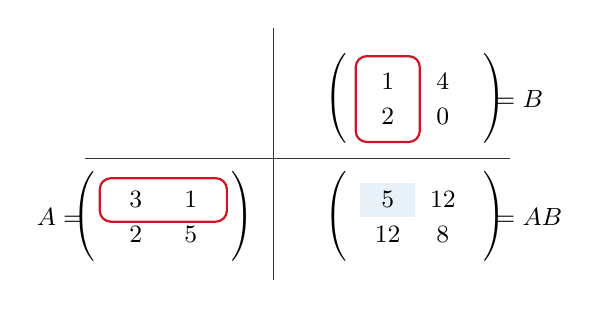
\begin{tikzpicture}[every node/.style={font=\small}]
  \matrix (B) [matrix of math nodes, left delimiter=(, right delimiter=), nodes={minimum width=7mm}] at (3.2,1.5)
    {1 & 4\\ 2 & 0\\};
  \matrix (A) [matrix of math nodes, left delimiter=(, right delimiter=), nodes={minimum width=7mm}] at (0,0)
    {3 & 1\\ 2 & 5\\};
  \matrix (C) [matrix of math nodes, left delimiter=(, right delimiter=), nodes={minimum width=7mm}] at (3.2,0)
    {|[fill=uimmlightblue]|5 & 12\\ 12 & 8\\};
  \draw[uimmgray] (1.4,2.4) -- (1.4,-0.8);
  \draw[uimmgray] (-1,0.75) -- (4.4,0.75);
  \node[left=2pt of A] {$A=$};
  \node[right=2pt of B] {$=B$};
  \node[right=2pt of C] {$=AB$};
  \draw[uimmred, thick, rounded corners] ($(A-1-1.north west)+(-0.1,0.05)$) rectangle ($(A-1-2.south east)+(0.1,-0.05)$);
  \draw[uimmred, thick, rounded corners] ($(B-1-1.north west)+(-0.05,0.1)$) rectangle ($(B-2-1.south east)+(0.05,-0.1)$);
\end{tikzpicture}
\end{center}
Coefficient encadré (ligne 1 de $A$, colonne 1 de $B$) : $3\times 1 + 1\times 2 = 5$.\\
Les autres : $c_{12}=3\times 4+1\times 0=12$ ; \ $c_{21}=2\times 1+5\times 2=12$ ; \ $c_{22}=2\times 4+5\times 0=8$.
\end{methode}

\begin{appliindus}[-- Fil rouge : besoins en composants et coût de la commande]\label{ex:besoins}
Notons $X = \M{40\\25\\10}$ la commande (colonne : $V_1$, $V_2$, $V_3$) et $P = \M{12{,}50 & 0{,}80 & 0{,}15}$ les prix unitaires (ligne : tige, joint, vis).

\textbf{1. Besoins.} $N$ est $3\times 3$, $X$ est $3\times 1$ : le produit $NX$ existe et il est $3\times 1$.
\[
NX = \M{1 & 1 & 2\\ 4 & 6 & 8\\ 8 & 8 & 12}\M{40\\25\\10}
= \M{1\times 40 + 1\times 25 + 2\times 10\\ 4\times 40 + 6\times 25 + 8\times 10\\ 8\times 40 + 8\times 25 + 12\times 10}
= \M{85\\390\\640}
\]
Il faut sortir $85$ tiges, $390$ joints et $640$ vis.

\textbf{2. Coût total.} $P$ est $1\times 3$, $NX$ est $3\times 1$ : le produit est un nombre ($1\times 1$).
\[
P(NX) = 12{,}50\times 85 + 0{,}80\times 390 + 0{,}15\times 640 = 1\,062{,}50 + 312 + 96 = 1\,470{,}50 \text{ €.}
\]

\textbf{3. Un autre chemin.} Le produit $PN$ ($1\times 3$) donne le coût en composants \textbf{de chaque vérin} :
\[
PN = \M{16{,}90 & 18{,}50 & 33{,}20}
\qquad\text{puis}\]
\[(PN)X = 16{,}90\times 40 + 18{,}50\times 25 + 33{,}20\times 10 = 1\,470{,}50 \text{ €.}
\]
On retrouve le même résultat : $P(NX) = (PN)X$. C'est l'\textbf{associativité} du produit. Le magasinier raisonne par composant, le chiffreur raisonne par vérin, et les deux tombent d'accord.
\end{appliindus}

\subsection{Propriétés du produit}\label{subsec:proprietes}

\begin{theoreme}[-- Règles de calcul]
Sous réserve que les produits existent :
\begin{itemize}
  \item \textbf{Associativité} : $(AB)C = A(BC)$ ; on écrit simplement $ABC$.
  \item \textbf{Distributivité} : $A(B+C) = AB + AC$ et $(A+B)C = AC + BC$.
  \item \textbf{Élément neutre} : si $A$ est carrée d'ordre $n$, $AI_n = I_nA = A$.
  \item \textbf{Réels} : $(kA)B = A(kB) = k(AB)$.
\end{itemize}
\end{theoreme}

\begin{attention}[-- Le produit n'est pas commutatif]\label{att:noncommut}
En général, $AB\neq BA$. Avec $A=\M{1 & 2\\ 0 & 1}$ et $B=\M{1 & 0\\ 3 & 1}$ :
\[
AB = \M{7 & 2\\ 3 & 1}
\qquad\text{mais}\qquad
BA = \M{1 & 2\\ 3 & 7}.
\]
Quand $AB$ existe, $BA$ peut même ne pas exister : avec $N$ ($3\times 3$) et $X$ ($3\times 1$), $NX$ existe mais $XN$ n'existe pas.\\
\textbf{Analogie atelier :} percer puis tarauder ne donne pas la même pièce que tarauder puis percer. L'ordre des opérations compte.
\end{attention}

\begin{attention}[-- Un produit nul sans facteur nul]\label{att:produitnul}
Avec $A=\M{1 & 2\\ 2 & 4}$ et $B=\M{2 & -4\\ -1 & 2}$ : \quad $AB = \M{0 & 0\\ 0 & 0}$ alors que ni $A$ ni $B$ n'est nulle.\\
La règle « un produit est nul si et seulement si l'un des facteurs est nul » est \textbf{fausse} pour les matrices. Conséquence : les identités remarquables ne s'appliquent plus telles quelles, car $(A+B)^2 = A^2 + AB + BA + B^2$, qui n'est pas $A^2+2AB+B^2$ en général.
\end{attention}

% ============================================================
\needspace{7cm}
\section{Puissances d'une matrice et processus discrets \hfill {\normalsize\color{uimmred}[S01] [C03]}}\label{sec:puissances}

\subsection{Définition}\label{subsec:defpuissance}

\begin{definition}[-- Puissance d'une matrice carrée]
Soit $A$ une matrice carrée et $n$ un entier naturel non nul. On note
\[
A^n = \underbrace{A\times A\times\cdots\times A}_{n \text{ facteurs}} \qquad\text{avec la convention}\qquad A^0 = I.
\]
Seules les matrices \textbf{carrées} ont des puissances (sinon $A\times A$ n'existe pas).
\end{definition}

\begin{exemple}[-- Un calcul à la main, puis une conjecture]\label{ex:puissance}
Soit $T = \M{1 & 1\\ 0 & 1}$.
\[
T^2 = \M{1 & 1\\ 0 & 1}\M{1 & 1\\ 0 & 1} = \M{1 & 2\\ 0 & 1}
\qquad
T^3 = T^2\,T = \M{1 & 2\\ 0 & 1}\M{1 & 1\\ 0 & 1} = \M{1 & 3\\ 0 & 1}.
\]
On conjecture $T^n = \M{1 & n\\ 0 & 1}$, ce que la calculatrice confirme pour $T^{10}$ ou $T^{50}$.
\end{exemple}

\begin{attention}
$A^2$ n'est \textbf{pas} la matrice des carrés des coefficients : $\M{1 & 1\\ 0 & 1}^2 = \M{1 & 2\\ 0 & 1}\neq\M{1 & 1\\ 0 & 1}$.
\end{attention}

\subsection{Calculer avec la calculatrice}\label{subsec:calculatrice}

\begin{methode}[-- Calculer $A^n$ à la calculatrice]
\begin{enumerate}
  \item Saisir la matrice $A$ (et la stocker dans une variable).
  \item Taper \texttt{A\^{}n} avec la valeur de $n$ voulue.
  \item Pour une suite $X_n = A^nX_0$, saisir aussi $X_0$ puis calculer \texttt{A\^{}n*X0}.
\end{enumerate}
Les manipulations détaillées pour les NumWorks, TI-83 Premium CE et Casio Graph 90+E sont regroupées dans la \textbf{fiche calculatrice en annexe}, p.~\pageref{fiche:calc}.
\end{methode}

\subsection{Processus discrets : suites de matrices}\label{subsec:processus}

\begin{theoreme}[-- Suite définie par $X_{n+1} = AX_n$]
Si une suite de matrices colonnes vérifie $X_{n+1} = AX_n$ pour tout entier $n$, alors
\[
\boxed{X_n = A^n X_0}
\]
\textbf{Analogie :} c'est l'équivalent matriciel d'une suite géométrique ($u_{n+1}=q\,u_n$ donne $u_n=q^n u_0$, voir MOD02).\\
\textbf{Justification :} $X_1 = AX_0$, $X_2 = AX_1 = A(AX_0) = A^2X_0$, $X_3 = AX_2 = A^3X_0$, et ainsi de suite.
\end{theoreme}

\begin{appliindus}[-- Disponibilité d'un parc de robots de soudage]\label{ex:robots}
Un site exploite $50$ robots de soudage. On relève leur état chaque lundi : en marche ($M$) ou en panne ($P$). L'historique de maintenance montre que, d'une semaine à la suivante :
\begin{itemize}
  \item un robot en marche le reste avec une probabilité $0{,}9$ et tombe en panne avec une probabilité $0{,}1$ ;
  \item un robot en panne est réparé (repasse en marche) avec une probabilité $0{,}6$ et reste en panne avec une probabilité $0{,}4$.
\end{itemize}
On note $m_n$ et $p_n$ les nombres moyens de robots en marche et en panne la semaine $n$, et $X_n = \M{m_n\\p_n}$. Au départ, tous les robots sont neufs : $X_0 = \M{50\\0}$.

\textbf{1. Mise en équation.} Les robots en marche la semaine $n+1$ viennent de deux sources :
\[
\left\{\begin{array}{l} m_{n+1} = 0{,}9\,m_n + 0{,}6\,p_n\\ p_{n+1} = 0{,}1\,m_n + 0{,}4\,p_n \end{array}\right.
\qquad\Longleftrightarrow\qquad
X_{n+1} = \underbrace{\M{0{,}9 & 0{,}6\\ 0{,}1 & 0{,}4}}_{A} X_n.
\]
\textbf{Lecture de $A$ :} la colonne 1 décrit le devenir d'un robot en marche, la colonne 2 celui d'un robot en panne. Chaque colonne a pour somme $1$ (un robot est forcément dans l'un des deux états).

\textbf{2. Calculs.} À la main : $X_1 = AX_0 = \M{0{,}9\times 50 + 0{,}6\times 0\\ 0{,}1\times 50 + 0{,}4\times 0} = \M{45\\5}$. À la calculatrice, $X_n = A^nX_0$ :
\begin{center}
\renewcommand{\arraystretch}{1.3}
\begin{tabular}{|c|c|c|c|c|c|c|}
\hline
\rowcolor{uimmlightblue}
$n$ & $0$ & $1$ & $2$ & $3$ & $5$ & $10$ \\
\hline
$m_n$ & $50$ & $45$ & $43{,}5$ & $43{,}05$ & $\approx 42{,}87$ & $\approx 42{,}86$ \\
\hline
$p_n$ & $0$ & $5$ & $6{,}5$ & $6{,}95$ & $\approx 7{,}13$ & $\approx 7{,}14$ \\
\hline
\end{tabular}
\end{center}
\textbf{3. Interprétation.} Le parc se stabilise très vite autour de $42{,}86$ robots en marche, soit une disponibilité d'environ $85{,}7\,\%$ (la valeur exacte est $\frac{6}{7}$). C'est l'indicateur qui sert à dimensionner le parc : pour disposer en moyenne de $45$ robots en marche, il faudrait environ $45\div\frac{6}{7}=52{,}5$, donc $53$ robots.
\end{appliindus}

\begin{remarque}[-- Convention ligne ou colonne]
Dans ce cours, l'état est une \textbf{colonne} et l'on écrit $X_{n+1} = AX_n$ (colonnes de somme $1$). Certains ouvrages utilisent un état en \textbf{ligne} et écrivent $L_{n+1} = L_nM$ (lignes de somme $1$). Les deux conventions donnent les mêmes résultats : il faut simplement rester cohérent du début à la fin.
\end{remarque}

\begin{appliindus}[-- Réseau de convoyeurs]\label{ex:reseau}
Un atelier comporte quatre postes : Débit ($D$), Usinage ($U$), Contrôle ($C$), Expédition ($E$). Des convoyeurs à sens unique relient certains postes :
\begin{center}
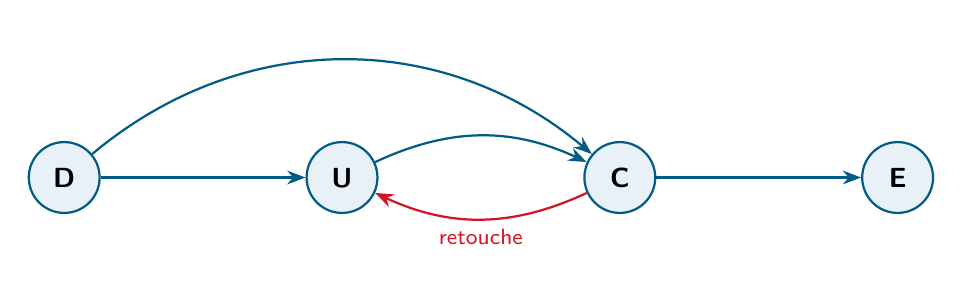
\begin{tikzpicture}[>=Stealth, node distance=2.6cm,
  poste/.style={circle, draw=uimmblue, fill=uimmlightblue, thick, minimum size=9mm, font=\bfseries}]
  \node[poste] (D) {D};
  \node[poste, right=of D] (U) {U};
  \node[poste, right=of U] (C) {C};
  \node[poste, right=of C] (E) {E};
  \draw[->, thick, uimmblue] (D) -- (U);
  \draw[->, thick, uimmblue] (U) to[bend left=25] (C);
  \draw[->, thick, uimmred] (C) to[bend left=25] node[below, font=\footnotesize] {retouche} (U);
  \draw[->, thick, uimmblue] (C) -- (E);
  \draw[->, thick, uimmblue] (D) to[bend left=40] (C);
\end{tikzpicture}
\end{center}
On note $G$ la matrice $4\times 4$ où $g_{ij}=1$ si un convoyeur va du poste $i$ au poste $j$, $0$ sinon (ordre $D$, $U$, $C$, $E$) :
\[
G = \M{0 & 1 & 1 & 0\\ 0 & 0 & 1 & 0\\ 0 & 1 & 0 & 1\\ 0 & 0 & 0 & 0}
\qquad\qquad
G^2 = \M{0 & 1 & 1 & 1\\ 0 & 1 & 0 & 1\\ 0 & 0 & 1 & 0\\ 0 & 0 & 0 & 0}\ \text{(calculatrice).}
\]
\textbf{Propriété admise :} le coefficient $(i,j)$ de $G^k$ est le \textbf{nombre de trajets en $k$ étapes} du poste $i$ au poste $j$.
\begin{itemize}
  \item $(G^2)_{14}=1$ : un seul trajet en deux étapes du débit à l'expédition ($D\to C\to E$).
  \item $(G^2)_{22}=1$ : une pièce peut revenir à l'usinage en deux étapes ($U\to C\to U$, boucle de retouche).
\end{itemize}
\end{appliindus}

% ============================================================
\needspace{7cm}
\section{Inverse d'une matrice carrée \hfill {\normalsize\color{uimmred}[S02] [C01] [C02]}}\label{sec:inverse}

\subsection{Motivation}\label{subsec:motivation}

Pour résoudre $3x = 12$, on multiplie par l'inverse de $3$ : $x = 3^{-1}\times 12 = 4$. On voudrait faire de même avec une équation matricielle $AX = B$. Mais on ne peut pas « diviser » par une matrice. On cherche donc une matrice qui joue le rôle de $\frac{1}{A}$ : c'est l'\textbf{inverse} de $A$.

\subsection{Définition et propriétés}\label{subsec:definverse}

\begin{definition}[-- Matrice inversible]
Soit $A$ une matrice carrée d'ordre $n$. On dit que $A$ est \textbf{inversible} s'il existe une matrice carrée $B$ d'ordre $n$ telle que
\[
AB = BA = I_n.
\]
\end{definition}

\begin{theoreme}[-- Unicité et commutativité]\label{th:unicite}
\begin{itemize}
  \item Si $A$ est inversible, la matrice $B$ est \textbf{unique}. On la note $A^{-1}$ et on l'appelle \textbf{l'inverse} de $A$.
  \item Une matrice inversible \textbf{commute} avec son inverse : $AA^{-1} = A^{-1}A = I_n$.
\end{itemize}
\textbf{Preuve de l'unicité.} Si $B$ et $B'$ conviennent toutes les deux : $B = BI_n = B(AB') = (BA)B' = I_nB' = B'$. On a utilisé l'associativité.
\end{theoreme}

\begin{methode}[-- Montrer que $B$ est l'inverse de $A$]\label{meth:montrerinverse}
On calcule le produit $AB$ et on vérifie qu'on obtient $I_n$. Pour des matrices carrées, on admet qu'un seul des deux produits suffit : si $AB=I_n$, alors $BA=I_n$ aussi.
\end{methode}

\begin{exemple}[-- Vérification à la main]\label{ex:verifinverse}
Montrons que $B=\M{3 & -1\\ -5 & 2}$ est l'inverse de $A=\M{2 & 1\\ 5 & 3}$.
\[
AB = \M{2\times 3 + 1\times(-5) & 2\times(-1) + 1\times 2\\ 5\times 3 + 3\times(-5) & 5\times(-1) + 3\times 2} = \M{1 & 0\\ 0 & 1} = I_2.
\]
Donc $A$ est inversible et $A^{-1} = \M{3 & -1\\ -5 & 2}$. (On peut vérifier que $BA = I_2$ aussi.)
\end{exemple}

\begin{attention}[-- Toutes les matrices carrées ne sont pas inversibles]\label{att:noninversible}
La matrice nulle n'est pas inversible ($0\times B = 0 \neq I$). La matrice $A=\M{1 & 2\\ 2 & 4}$ non plus : sa ligne 2 est le double de sa ligne 1, donc, pour toute matrice $B$, la ligne 2 de $AB$ est le double de la ligne 1 de $AB$. Or la ligne 2 de $I_2$, $\M{0 & 1}$, n'est pas le double de sa ligne 1, $\M{1 & 0}$. Aucune matrice $B$ ne vérifie $AB = I_2$.\\
Le programme n'exige aucune condition d'inversibilité : en pratique, \textbf{la calculatrice signale} une matrice non inversible (message d'erreur du type « matrice singulière »).
\end{attention}

\subsection{Calcul de l'inverse}\label{subsec:calculinverse}

\begin{methode}[-- Déterminer l'inverse à la calculatrice]\label{meth:inversecalc}
On saisit la matrice puis on utilise la touche $x^{-1}$ (voir la fiche calculatrice p.~\pageref{fiche:calc}). On \textbf{vérifie} ensuite le résultat en calculant $A\times A^{-1}$.
\end{methode}

\begin{exemple}[-- Inverse de la nomenclature du fil rouge]\label{ex:inverseN}
La calculatrice donne, pour $N=\M{1 & 1 & 2\\ 4 & 6 & 8\\ 8 & 8 & 12}$ :
\[
N^{-1} = \M{-1 & -\frac{1}{2} & \frac{1}{2}\\[2pt] -2 & \frac{1}{2} & 0\\[2pt] 2 & 0 & -\frac{1}{4}}
= \M{-1 & -0{,}5 & 0{,}5\\ -2 & 0{,}5 & 0\\ 2 & 0 & -0{,}25}.
\]
Contrôle : la calculatrice affiche bien $N\times N^{-1} = I_3$.
\end{exemple}

\begin{horsprog}[-- Formule de l'inverse d'une matrice $2\times 2$]\label{hp:formule}
Pour $A=\M{a & b\\ c & d}$, on pose $\Delta = ad - bc$ (le \textbf{déterminant} de $A$). Si $\Delta\neq 0$, alors
\[
A^{-1} = \frac{1}{ad-bc}\M{d & -b\\ -c & a}.
\]
Si $\Delta = 0$, $A$ n'est pas inversible. \textbf{Exemple :} pour $A=\M{2 & 1\\ 5 & 3}$, $\Delta = 6-5 = 1$ et l'on retrouve $A^{-1}=\M{3 & -1\\ -5 & 2}$. Pour $\M{1 & 2\\ 2 & 4}$, $\Delta = 4 - 4 = 0$.\\
\textit{Cette formule n'est pas exigible en BTS : elle permet seulement de contrôler un résultat.}
\end{horsprog}

\begin{remarque}[-- Les puissances négatives]
Si $A$ est inversible, on note $A^{-2} = (A^{-1})^2$, etc. Et si $A$ est inversible, la solution de $AX = AY$ est $X = Y$ (on multiplie à gauche par $A^{-1}$) : on peut « simplifier » par une matrice inversible, pas par une matrice quelconque.
\end{remarque}

% ============================================================
\needspace{7cm}
\section{Résolution de systèmes linéaires \hfill {\normalsize\color{uimmred}[S02] [C03]}}\label{sec:systemes}

\subsection{Écriture matricielle d'un système}\label{subsec:ecriture}

\begin{definition}[-- Forme matricielle $AX=B$]
Le système de $n$ équations à $n$ inconnues
\[
\left\{\begin{array}{l}
a_{11}x_1 + a_{12}x_2 + \cdots + a_{1n}x_n = b_1\\
\quad\vdots\\
a_{n1}x_1 + a_{n2}x_2 + \cdots + a_{nn}x_n = b_n
\end{array}\right.
\quad\text{s'écrit}\quad
AX = B
\]
\[
\text{avec}\quad
A = (a_{ij}),\qquad X=\M{x_1\\ \vdots\\ x_n},\qquad B=\M{b_1\\ \vdots\\ b_n}.
\]
$A$ est la \textbf{matrice du système} (coefficients des inconnues), $X$ la colonne des \textbf{inconnues}, $B$ la colonne des \textbf{seconds membres}.
\end{definition}

\begin{theoreme}[-- Résolution par inversion]\label{th:resolution}
Si $A$ est inversible, le système $AX=B$ admet une \textbf{unique} solution :
\[
\boxed{X = A^{-1}B}
\]
\textbf{Preuve.} On multiplie les deux membres \textbf{à gauche} par $A^{-1}$ : $A^{-1}(AX) = A^{-1}B$, soit $(A^{-1}A)X = A^{-1}B$, soit $I_nX = X = A^{-1}B$.
\end{theoreme}

\begin{attention}
$X = A^{-1}B$ et \textbf{non} $BA^{-1}$. Avec $B$ de format $n\times 1$ et $A^{-1}$ de format $n\times n$, le produit $BA^{-1}$ n'existe d'ailleurs pas. Le programme se limite aux systèmes où $A$ est inversible (systèmes « de Cramer »), sans justification demandée.
\end{attention}

\begin{methode}[-- Résoudre un système par inversion, en 4 étapes]\label{meth:systeme}
\begin{enumerate}
  \item \textbf{Nommer} les inconnues (avec leur unité) et \textbf{écrire} le système.
  \item \textbf{Traduire} en $AX=B$ : écrire $A$, $X$, $B$ en gardant le même ordre des inconnues dans chaque équation.
  \item \textbf{Calculer} $X = A^{-1}B$ : à la main à l'ordre 2 si $A^{-1}$ est donnée, à la calculatrice sinon.
  \item \textbf{Vérifier} (remplacer dans une équation) et \textbf{conclure} par une phrase avec les unités.
\end{enumerate}
\end{methode}

\begin{appliindus}[-- Plan de charge de deux machines (ordre 2, à la main)]\label{ex:plancharge}
Un atelier fabrique deux pièces, $A$ et $B$. Une pièce $A$ demande $2$\,h de tournage et $5$\,h de fraisage ; une pièce $B$ demande $1$\,h de tournage et $3$\,h de fraisage. Ce mois-ci, le tour est disponible $100$\,h et la fraiseuse $270$\,h. Combien de pièces de chaque type fabriquer pour saturer les deux machines ?

\textbf{1.} Soit $x$ le nombre de pièces $A$ et $y$ le nombre de pièces $B$.
\qquad
$\left\{\begin{array}{ll} 2x + y = 100 & \text{(tournage)}\\ 5x + 3y = 270 & \text{(fraisage)}\end{array}\right.$

\textbf{2.} $\M{2 & 1\\ 5 & 3}\M{x\\y} = \M{100\\270}$, soit $AX = B$.

\textbf{3.} On a montré (exemple p.~\pageref{ex:verifinverse}) que $A^{-1}=\M{3 & -1\\ -5 & 2}$. Donc
\[
X = A^{-1}B = \M{3 & -1\\ -5 & 2}\M{100\\270} = \M{300 - 270\\ -500 + 540} = \M{30\\40}.
\]
\textbf{4.} Vérification : $2\times 30 + 40 = 100$ et $5\times 30 + 3\times 40 = 270$. Il faut fabriquer $30$ pièces $A$ et $40$ pièces $B$.

\textbf{Intérêt de la méthode :} si les disponibilités changent (congés, panne), il suffit de refaire le produit $A^{-1}B$ avec le nouveau $B$. L'inverse, lui, ne change pas.
\end{appliindus}

\begin{appliindus}[-- Fil rouge : vider le stock (ordre 3, à la calculatrice)]\label{ex:stock}
Le stock contient $85$ tiges, $390$ joints et $640$ vis. On cherche le nombre $x_1$, $x_2$, $x_3$ de vérins $V_1$, $V_2$, $V_3$ qui consomme exactement ce stock. D'après la nomenclature :
\[
\left\{\begin{array}{l} x_1 + x_2 + 2x_3 = 85\\ 4x_1 + 6x_2 + 8x_3 = 390\\ 8x_1 + 8x_2 + 12x_3 = 640\end{array}\right.
\quad\Longleftrightarrow\quad
NX = S \quad\text{avec}\quad S = \M{85\\390\\640}.
\]
Avec $N^{-1}$ calculée p.~\pageref{ex:inverseN} :
\[
X = N^{-1}S = \M{-1 & -0{,}5 & 0{,}5\\ -2 & 0{,}5 & 0\\ 2 & 0 & -0{,}25}\M{85\\390\\640} = \M{40\\25\\10}.
\]
On assemble $40$ vérins $V_1$, $25$ vérins $V_2$ et $10$ vérins $V_3$. C'est la commande de départ : le calcul « remonte » des composants aux produits, en sens inverse du paragraphe~\ref{sec:produit}. \textbf{$N$ va des vérins vers les composants, $N^{-1}$ revient des composants vers les vérins.}
\end{appliindus}

% ============================================================
\newpage
\section{Synthèse}\label{sec:synthese}

\subsection{Carte mentale du module}\label{subsec:carte}

\begin{center}
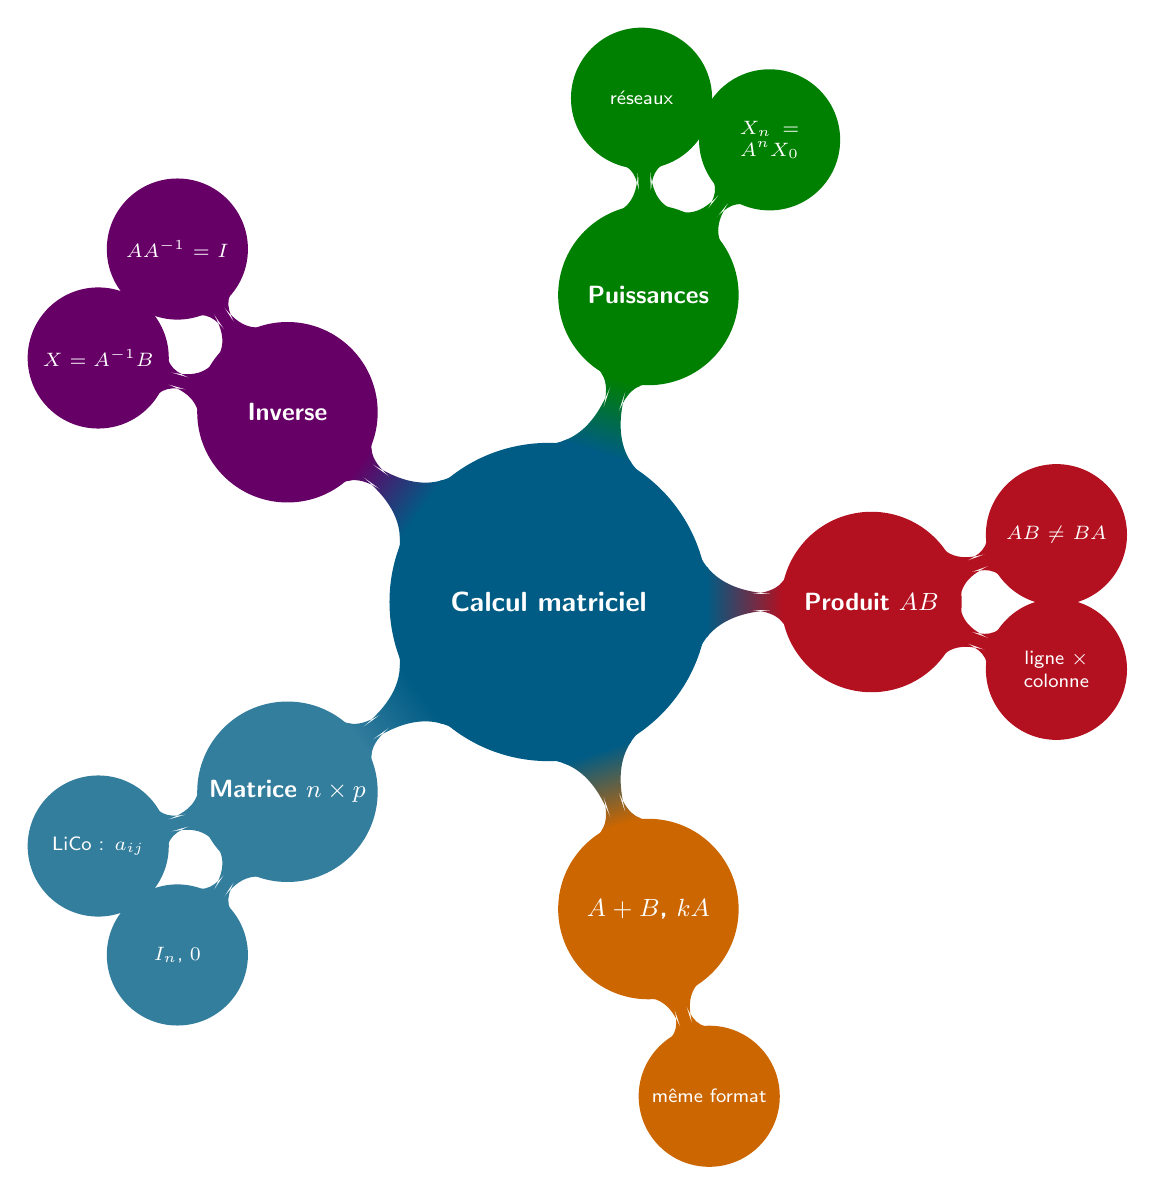
\begin{tikzpicture}[mindmap, grow cyclic, every node/.style={concept, execute at begin node=\hskip0pt},
  concept color=uimmblue, text=white, font=\sffamily\bfseries,
  level 1/.append style={level distance=4.1cm, sibling angle=72, font=\sffamily\small\bfseries},
  level 2/.append style={level distance=2.5cm, sibling angle=40, font=\sffamily\scriptsize}]
\node[font=\sffamily\bfseries] {Calcul matriciel}
  child[concept color=uimmblue!80] { node {Matrice $n\times p$}
    child { node {LiCo : $a_{ij}$} }
    child { node {$I_n$, $0$} } }
  child[concept color=orange!80!black] { node {$A+B$, $kA$}
    child { node {même format} } }
  child[concept color=uimmred!85!black] { node {Produit $AB$}
    child { node {ligne $\times$ colonne} }
    child { node {$AB\neq BA$} } }
  child[concept color=green!50!black] { node {Puissances}
    child { node {$X_n=A^nX_0$} }
    child { node {réseaux} } }
  child[concept color=violet!80!black] { node {Inverse}
    child { node {$AA^{-1}=I$} }
    child { node {$X=A^{-1}B$} } };
\end{tikzpicture}
\end{center}

\subsection{Les erreurs fréquentes}\label{subsec:erreurs}

\begin{center}
\renewcommand{\arraystretch}{1.4}
\begin{tabular}{|p{6.8cm}|p{8.6cm}|}
\hline
\rowcolor{uimmlightblue}
\textbf{Erreur} & \textbf{Ce qu'il faut faire} \\
\hline
Multiplier coefficient par coefficient pour $AB$ & Ligne de $A$ par colonne de $B$, puis additionner. \\
\hline
Écrire $AB = BA$ & L'ordre compte : garder l'ordre de l'énoncé. \\
\hline
Calculer $A^2$ en élevant chaque coefficient au carré & $A^2 = A\times A$ (produit matriciel). \\
\hline
Écrire $X = BA^{-1}$ ou $X = \frac{B}{A}$ & $X = A^{-1}B$ : on multiplie \textbf{à gauche} par $A^{-1}$. \\
\hline
Mélanger l'ordre des inconnues entre deux équations & Écrire toutes les équations avec les inconnues dans le même ordre avant de former $A$. \\
\hline
Oublier de vérifier l'inverse fourni par la calculatrice & Calculer $AA^{-1}$ : on doit trouver $I_n$. \\
\hline
\end{tabular}
\end{center}

\subsection{Regards croisés : trois professionnels, une même matrice}\label{subsec:regards}

\begin{remarque}[-- Table ronde]
\begin{itemize}
  \item \textbf{Le technicien méthodes :} « Ma nomenclature et ma gamme sont des matrices. Un produit matriciel me donne la charge de chaque machine pour toute la commande, en une seule opération dans le tableur. »
  \item \textbf{Le responsable maintenance :} « Avec la matrice de transition de mon parc, je prévois la disponibilité à 10 semaines. La puissance $A^n$ me dit vers quoi le parc se stabilise. »
  \item \textbf{L'automaticien :} « Chaque mouvement d'un robot est une matrice de rotation ou de changement de repère. Enchaîner deux mouvements, c'est multiplier deux matrices, et l'ordre compte : c'est pour cela que $AB\neq BA$. »
\end{itemize}
\end{remarque}

\needspace{12cm}\subsection{Testez-vous}\label{subsec:quiz}

\begin{exemple}[-- Quiz d'auto-évaluation (réponses en bas de page)]
\begin{enumerate}
  \item $A$ est $2\times 3$ et $B$ est $3\times 4$. Quel est le format de $AB$ ? Le produit $BA$ existe-t-il ?
  \item Calculer $\M{1 & 2\\ 3 & 4}\M{1\\ -1}$.
  \item Vrai ou faux : si $AB=0$, alors $A=0$ ou $B=0$.
  \item Que vaut $AI_3$ pour $A$ carrée d'ordre 3 ?
  \item On sait que $\M{1 & 1\\ 1 & 2}^{-1} = \M{2 & -1\\ -1 & 1}$. Résoudre $\left\{\begin{array}{l}x+y=5\\ x+2y=8\end{array}\right.$
  \item Une suite vérifie $X_{n+1}=AX_n$. Exprimer $X_{12}$ en fonction de $X_0$.
\end{enumerate}
\vspace{2pt}
\rule{\linewidth}{0.4pt}\\
\footnotesize\textit{Réponses.} 1. $2\times 4$ ; non ($4\neq 2$). \ 2. $\M{-1\\-1}$. \ 3. Faux (voir p.~\pageref{att:produitnul}). \ 4. $A$. \ 5. $\M{x\\y}=\M{2 & -1\\ -1 & 1}\M{5\\8}=\M{2\\3}$. \ 6. $X_{12}=A^{12}X_0$.
\end{exemple}

\subsection{Plan de travail conseillé}\label{subsec:plan}

\begin{center}
\renewcommand{\arraystretch}{1.35}
\begin{tabular}{|c|p{6.5cm}|p{7.5cm}|}
\hline
\rowcolor{uimmlightblue}
\textbf{Étape} & \textbf{Cours} & \textbf{TD (exercices)} \\
\hline
1 & §\ref{sec:notion} et §\ref{sec:addition} : lire une matrice, additionner & Exercices 1 et 2 \\
\hline
2 & §\ref{sec:produit} : produit matriciel & Exercices 3 à 7 \\
\hline
3 & §\ref{sec:puissances} : puissances, processus discrets & Exercices 8 à 10 (calculatrice) \\
\hline
4 & §\ref{sec:inverse} : inverse & Exercices 11 et 12 \\
\hline
5 & §\ref{sec:systemes} : systèmes & Exercices 13 à 16, puis le problème de synthèse \\
\hline
\end{tabular}
\end{center}

\begin{remarque}[-- Pour progresser]
Après chaque exercice, notez dans la marge le type d'erreur commise (format, ordre du produit, calcul, interprétation). Au bout de trois exercices, la même étiquette qui revient désigne le point à retravailler en priorité.
\end{remarque}

% ============================================================
\newpage
\section*{Annexe -- Fiche calculatrice}\label{sec:annexe}
\addcontentsline{toc}{section}{Annexe -- Fiche calculatrice}

\begin{calculatrice}[-- Matrices : saisie, produit, puissance, inverse]\label{fiche:calc}
\small
\renewcommand{\arraystretch}{1.35}
\begin{tabular}{@{}>{\bfseries\color{uimmblue}}p{1.8cm}|p{4.35cm}|p{4.35cm}|p{4.35cm}@{}}
 & \textbf{NumWorks} & \textbf{TI-83 Premium CE} & \textbf{Casio Graph 90+E} \\
\hline
Saisir $A$ &
Application \textit{Calculs}. \touche{boîte à outils} puis \textit{Matrices et vecteurs} $\rightarrow$ \textit{Matrice}. Remplir le gabarit (les flèches ajoutent lignes et colonnes). Stocker avec \touche{sto$\rightarrow$} dans la variable \texttt{A}. &
\touche{2nde}\touche{$x^{-1}$} (menu \textit{matrice}), onglet \textit{EDIT}, choisir \texttt{[A]}, saisir le format ($n\times p$) puis les coefficients. Quitter : \touche{2nde}\touche{mode}. &
Menu \textit{Exe-Mat}, touche de fonction \textit{MAT/VCT}. Choisir \texttt{Mat A}, saisir le format puis les coefficients. Retour : \touche{EXIT}. \\
\hline
Appeler $A$ &
Taper \texttt{A} (\touche{alpha} puis la lettre). &
\touche{2nde}\touche{$x^{-1}$}, onglet \textit{NOMS}, \texttt{[A]}. &
\touche{OPTN} $\rightarrow$ \textit{MAT/VCT} $\rightarrow$ \textit{Mat}, puis \touche{ALPHA} et la lettre. \\
\hline
$AB$, $A+B$, $kA$ & \texttt{A*B}, \texttt{A+B}, \texttt{3*A} & \texttt{[A]*[B]}, \texttt{[A]+[B]} & \texttt{Mat A * Mat B} \\
\hline
$A^{n}$ & \texttt{A\^{}10} & \texttt{[A]\^{}10} & \texttt{Mat A \^{} 10} \\
\hline
$A^{-1}$ & \texttt{A\^{}-1} ou \texttt{inverse(A)} & \texttt{[A]} puis \touche{$x^{-1}$} & \texttt{Mat A} puis \touche{SHIFT}\touche{)} ($x^{-1}$) \\
\hline
$X=A^{-1}B$ & \texttt{A\^{}-1*B} & \texttt{[A]}\touche{$x^{-1}$}\texttt{*[B]} & \texttt{Mat A$^{-1}$ * Mat B} \\
\end{tabular}

\smallskip
\footnotesize\textit{Les intitulés des menus peuvent varier légèrement selon la version du système. Pour afficher des fractions : NumWorks les donne directement ; TI : \touche{math} \texttt{1:$\blacktriangleright$Frac} ; Casio : touche \touche{S$\Leftrightarrow$D}.}
\end{calculatrice}

\begin{remarque}[-- Contrôler la calculatrice]
Après chaque calcul d'inverse, vérifier que $A\times A^{-1}$ affiche $I_n$. Des valeurs comme $1{,}2\times 10^{-13}$ à la place de $0$ sont des erreurs d'arrondi de la machine : on les lit comme $0$.
\end{remarque}

\end{document}
